\chapter{Метод оценки линейного искажающего оператора}
\section{Нахождение параметров искажения}
Как было сказано ранее, для восстановления изображения необходимо определить искажающий оператор. Он представляется дискретной импульсной характеристикой(ИХ). Однако такое представление не самое удачное для поиска, потому что имеет слишком большое количестве степеней свободы. Для эффективного поиска необходимо построить более удобную модель, задающую оператор ограниченным количеством параметров.

ИХ для вычислений представляется в виде матрицы. Простейшее представление смаза~--- линейный смаз~(\ref{eq:horizontalBlurPsf}).
\begin{equation}\label{eq:linearBlurArray}
\begin{pmatrix}
0 & 0 & 0 & 0.092 & 0.024\\
0 & 0.22 & 0.181 & 0.213 & 0.024\\
0.121 & 0.255 & 0.038 & 0 & 0\\
0.061 & 0 & 0 & 0 & 0
\end{pmatrix}
\end{equation}

Так например представляется в ИХ смаза длиной в 5 пикселей под углом $30^\circ$
\subsection{Кепстральный метод оценки линейного оператора}
Линейный смаз представляется величиной и углом смаза, альтернативное представление: координаты вектора смаза. Как уже было сказано ранее в разделе~(\ref{seqtion:distortionModel}) по спектру искажённого изображения визуально можно определить величину и угол смаза.
\begin{figure}[h!]
	\centering
	\begin{subfigure}[t]{0.3\textwidth}
		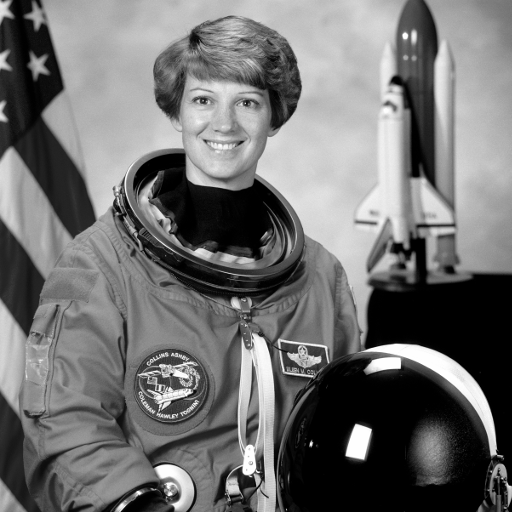
\includegraphics[width=\linewidth]{astro}
		\caption{исходное изображение}
	\end{subfigure}
	\hfill
	\begin{subfigure}[t]{0.3\textwidth}
		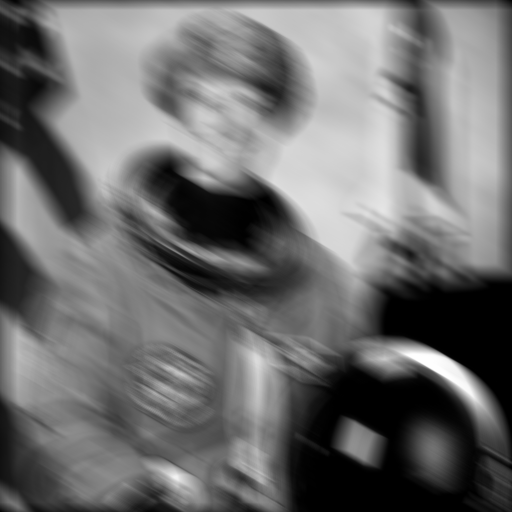
\includegraphics[width=\linewidth]{deconv-astro-blurred-shift40}
		\caption{смазанное изображение}
		\label{fig:astroShift40}
	\end{subfigure}%
	\hfill
	\begin{subfigure}[t]{0.3\textwidth}
		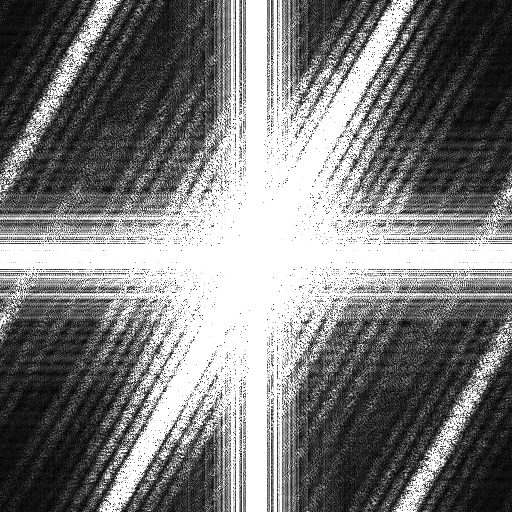
\includegraphics[width=\linewidth]{deconv-astro-spectre-shift40}
		\caption{спектр смазанного изображения}
		\label{fig:astroShift40Spectre}
	\end{subfigure}
	\caption{Смаз величиной в 40 пикселей под углом $330^{\circ}$}
	\label{fig:spectre}
\end{figure}

На рисунке~\ref{fig:spectre} представлены оригинальное изображение, исходное изображение подвергнутое смазу и спектр смазанного изображения. По спектру \ref{fig:astroShift40Spectre} расстояние между чёрными полосами, в которых значение спектра близко к нулю является обратным к величине смаза. Данные полосы ортогональны вектору смаза, угол наклона которого равен $330^\circ$. Однако, определение точных значений этих величин по частотному представлению изображения затруднительно. Для корректной работы методов восстановления изображения важно как можно точнее оценить ФРТ. Поэтому используют более точные способы определения параметров смаза.

Один из таких методов оценки параметров оператора линейного смаза основан на использовании кепстра изображения $\hat{f}(x,y)$~\cite{iterableImageRestorationBiemonLangdeik}
\begin{definition}\label{def:kepstr}
	\textbf{Кепстром} $\hat{f}(x,y)$ изображения называют обратное преобразование Фурье логарифма модуля преобразования Фурье.
	\begin{equation}
	\hat{g}(x,y) = F^{-1}\{log|F(u,v)|\},
	\end{equation}
\end{definition}
где $F^{-1}\{\cdot\}$~--- обратное преобразование Фурье, а $F(u,v)$~--- частотное представление изображения. Название <<кепстр>> получено перестановкой первых четырёх букв слова <<спектр>>.

Одним из основных свойств кепстра является то, что при свёртке двух сигналов их кепстры складываются. Таким образом, если
\begin{equation}
	g(x,y) = h(x,y) \conv f(x,y),
\end{equation}
то \cite{iterableImageRestorationBiemonLangdeik}
\begin{equation}\label{eq:kepstrSum}
	\hat{g}(x,y) = \hat{h}(x,y) + \hat{f}(x,y)
\end{equation}

При горизонтальном размытии ЧХ искажения можно записать в виде~(\ref{eq:horizontalBlurIRFourier}):
\begin{equation*}
H(u,v) =       
\frac{1}{L+1}e^{-i\frac{L\pi}{N}m}\frac{\sin\frac{\pi(L+1)u}{N}}{\sin\frac{\pi u}{N}}
\end{equation*}

Она имеет нули в точках $\frac{N}{L+1}k, v$, где $k$~--- ненулевое целое, поэтому $\hat{h}(x,y)$ имеет большой отрицательный пик на расстоянии $L$ от начала координат. Следовательно у кепстра искажённого изображения он тоже будет, что сообщает о наличии искажения и его параметрах.
\begin{figure}[h!]
	\centerline{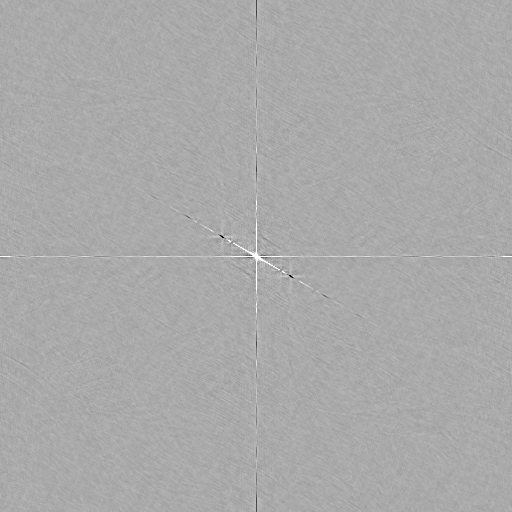
\includegraphics[width=0.5\linewidth]{deconv-kepstr-shift40-pi6}}
	\caption{Кепстр изображения смазанного на 40 пикселей под углом $330^{\circ}$.}
	\label{fig:kepstr}
\end{figure}

На рисунке~\ref{fig:kepstr} изображён кепстр искажённого изображения~\ref{fig:astroShift40}. В центре находится точка $(0,0)$. Симметрично относительно неё расположены тёмные точки, соответствующие отрицательным пикам, характеризующим параметры смаза. Их координаты соответствуют вектору смаза. Таким образом можно достаточно точно определить искажение. Отклонение от реальных значений достигает 1-2 пикселей.

\begin{figure}[h!]
	\centerline{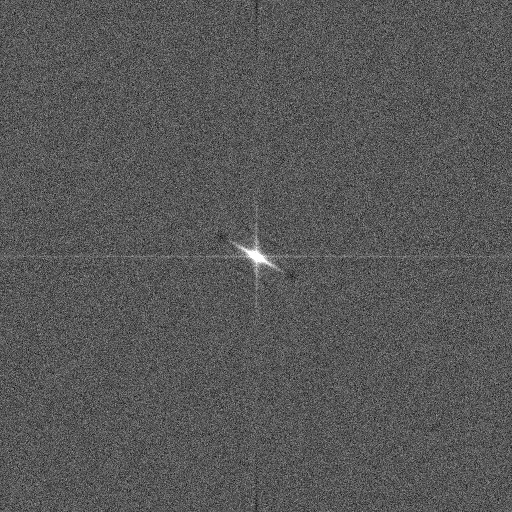
\includegraphics[width=0.5\linewidth]{deconv-kepstr-noised-shift40-pi6}}
	\caption{Кепстр изображения смазанного на 40 пикселей под углом $330^{\circ}$, зашумлённого с $\sigma=0,1$.}
	\label{fig:kepstrNoised}
\end{figure}
%%%% сослаться на диплом Кристины? Не это: ~\cite{panfilovaLinearBlur}
Кепстральный метод обладает рядом недостатков: в случае небольшого искажения (длина вектора размытия меньше 5 пикселей), точное определения смаза становится затруднительным. Также проблематично определить вектор смаза при большом шуме($\sigma_\eta \geq 5\cdot 10^{-2}$)\cite{panfilovaThesis} Так как вклад шума слишком велик, минимум спектра приходится на случайную составляющую спектра, что видно на рисунке~\ref{fig:kepstrNoised}.

\subsection{Уточнение параметров искажения}
Кепстральный метод находит только целочисленные координаты вектора сдвига с погрешностью в несколько пикселей, тогда как на практике величина смаза есть число вещественное. Ниже будет рассмотрен алгоритм позволяющий уточнить параметры смаза.

Найти наилучшую оценку искажающего оператора~\ref{def:bestPsfEstimaton} невозможно, так как исходное изображение в общем случае неизвестно. Вместо этого можно минимизировать целевую функцию, а именно MSE конволюции оценки изображения и искажающего оператора относительно искажённого изображения. Тогда искомая ИХ $\hat{h}^*$ будет найдена по следующей формуле:
\begin{equation}\label{eq:bestPsfModified}
\hat{h}^* = \argmin_{\hat{h}} MSE(g, \phi(g,\hat{h}) \conv \hat{h}),
\end{equation}
где $\phi(g, h)$~--- результат применения деконволюции(используем метод Люси-Ричардсона) с оператором $h$.

Так как ИХ линейного смаза $h_{x_h,y_h}(x,y)$описывается координатами вектора смаза, минимизировать будем функцию двух переменных $x_h, y_h$.

%%%%%%%%%%%%%%%%%%%%%%%%%%%%%%%%%%%%%%%%%%%%%%%%%%%%%%%%
\section{Нахождение параметров криволинейного искажающего оператора}

\subsection{Представление криволинейного искажающего оператора}
Представление смаза отрезком~--- удобно, но не всегда отражает действительность. В общем случае смаз криволинеен.

\begin{figure}[h!]
	\centering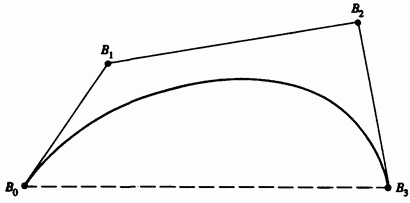
\includegraphics[width=0.5\linewidth]{bezier-curve-polygon-from-book}
	\caption{Кривая Безье и определяющие её точки.}
	\label{fig:bezierPolygon}
\end{figure}

Пьер Безье предложил метод создания кривых и поверхностей любой формы. Безье вывел математическую основу своего метода из геометрических соображений. Кривая Безье задаётся многоугольником как показано на рисунке~\ref{fig:bezierPolygon}.~\cite{mathBasicsOfCopmuterGraphics}.
Математическое представление кривой Безье имеет вид:
\begin{equation}
P(t) = \sum_{i=0}^{n} B_i J_{n,i}(t),\ 0\leq t \leq 1,
\label{eq:bezierCurveN}
\end{equation}
где $B_i, i=0\dots n-1$~--- точки многоугольника Безье, $J_{n,i}(t)$~--- базис Безье или Бернштейна, или функция аппроксимации:
\begin{equation*}
J_{n,i}(t) = \begin{pmatrix}
n \\ i
\end{pmatrix} t^i (1-t)^{n-i}
\end{equation*}
\begin{equation*}
\begin{pmatrix}
n \\ i
\end{pmatrix} = \frac{n!}{i!(n-i)!}
\end{equation*}

Так как обычно за время спуска затвора не проходит много времени, то движение не является сложным, поэтому криволинейный смаз будем представлять кривой Безье второго порядка. Она строится по трём точкам и будет иметь вид~(\ref{eq:bezierCurveN}):
\begin{equation}
	\begin{aligned}
	P(t) & = B_0 J_{2,0} + B_1 J_{2,1} + B_2 J_{2,2} = \\
		 & = (1-t)^2 P_0 + 2t(1-t)P_1+t^2 P_2
	\end{aligned}
	\label{eq:bezierCurve2}
\end{equation}
\begin{figure}[h!]
	\begin{subfigure}[t]{0.3\textwidth}
		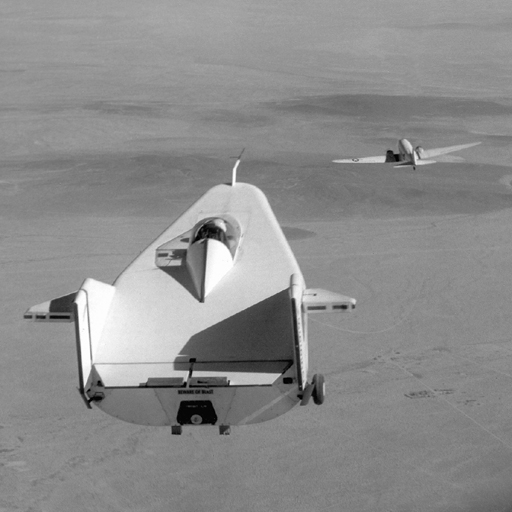
\includegraphics[width=\linewidth]{../liftingbody}
		\caption{Исходное изображение}
		\label{fig:liftingCurvedOriginal}
	\end{subfigure}
	\hfill
	\begin{subfigure}[t]{0.3\textwidth}
		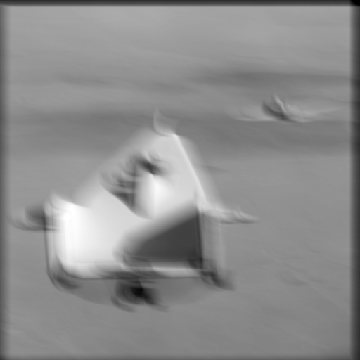
\includegraphics[width=\linewidth]{one-dim-iterated-blurred-data}
		\caption{смазанное изображение}
		\label{fig:liftingCurvedBlurred}
	\end{subfigure}
	\hfill
	\begin{subfigure}[t]{0.3\textwidth}
		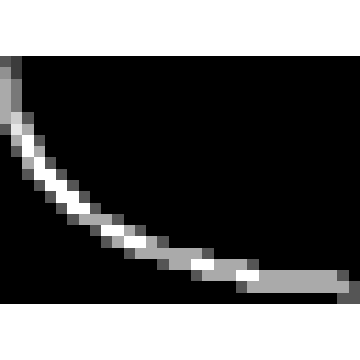
\includegraphics[width=\linewidth]{one-dim-iterated-curved-psf-real}
		\caption{кривая Безье второго порядка, построенной по точкам $B_0=(0; 0), B_1=(1; 18), B_2=(30; 20)$}
		\label{fig:curvedPsf}
	\end{subfigure}
	\caption{Смаз изображения криволинейным оператором}
\end{figure}

На рисунке~\ref{fig:curvedPsf} показана импульсная характеристика искажающего оператора представленная кривой Безье второго порядка, а на рисунке \ref{fig:liftingCurvedBlurred} изображение смазанное, этим оператором

\subsection{Первое приближение}
\begin{figure}[h!]
	\begin{subfigure}[t]{0.5\textwidth}
		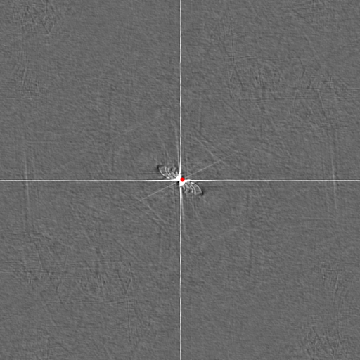
\includegraphics[width=\linewidth]{one-dim-iterated-kepstr}
		\caption{кепстр изображения \ref{fig:liftingCurvedBlurred}}
		\label{fig:curvedKepstrUnmodified}
	\end{subfigure}
	\begin{subfigure}[t]{0.5\textwidth}
		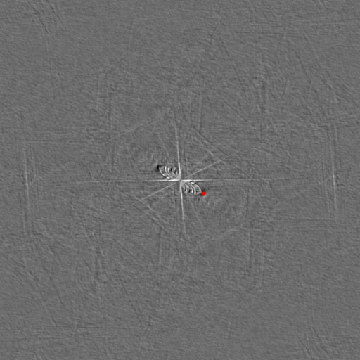
\includegraphics[width=\linewidth]{one-dim-iterated-kepstr-with-guass}
		\caption{сумма кепстра изображения \ref{fig:liftingCurvedBlurred} и гауссовой маски с $\sigma=3$}
		\label{fig:curvedKepstrWithGauss}
	\end{subfigure}
	\caption{Кепстр изображения с выделенным минимумом}
	\label{fig:}
\end{figure}

Итак будем приближать искажающий оператор кривой Безье второго порядка. Следовательно для полного задания оператора достаточно определить координаты трёх точек $B_0, B_1, B_2$ задающих кривую. Так как искажение инвариантно к смещению, то первую точку зафиксируем в нуле $B_0 = (0;0)$.

Точку $B_2$ попробуем приблизить применив метод из предыдущего раздела. Посмотрев на рисунок \ref{fig:curvedKepstrUnmodified} визуально можно определить минимумы в тёмных точках вблизи нуля и на определённом расстоянии. Однако абсолютный минимум(отмечен красной точкой) вблизи нуля не является искомой точкой. Чтобы исключить некорректные минимумы прибавим к кепстру ядро Гаусса~(\ref{eq:gaussKernel}).
\begin{equation}\label{eq:gaussKernel}
	gauss(x,y) = \frac{1}{\sigma\sqrt{2\pi}}e^{-\frac{x^2+y^2}{2\sigma^2}},
\end{equation}
где $\sigma$~--- масштабирующий параметр выбираемый эмпирически.

На сумме кепстра и ядра Гаусса(рисунок \ref{fig:curvedKepstrWithGauss}) корректно обнаруживается минимум, соответствующий кривой $B_2=(x_3,y_3)$. Первое приближение точки $B_1$ можно поместить посередине полученного отрезка.

\subsection{Второе приближение}
Для оценки $B_1$ построим целевую функцию $\psi(x,y)$ и будем её минимизировать. В качестве целевой функции возьмём:
\begin{equation}\label{eq:costFunction}
	\psi(x_2,y_2) = \left\|g - \phi(g, \hat{h}_{x_2,y_2}) \conv \hat{h}_{x_2,y_2}\right\|^2,
\end{equation}
где $h_{x_2,y_2}$~--- искажающий оператор представляющий собой кривую Безье построенную по точкам $b_0=(0;0), B_1=(x_2;y_2), B_2=(x_3;y_3)$. Здесь $x_3, y_3$~--- координаты третьей точки полученные путём анализа кепстра, см. предыдущий подраздел. Таким образом будем выбирать такой искажающий оператор, чтобы изображение восстановленное с его помощью и затем искажённое им же было наиболее похожим на входное смазанное изображение.

Однако данная целевая функция имеет множество локальных минимумов что можно увидеть на рис.~\ref{fig:costFunctionGrid}(темнее~--- значение меньше), где изображена целевая функция для кривой Безье $B_0=(0;0), B_1=(15;4), B_2=(20, 20)$. Поэтому классические градиентные методы здесь плохо применимы.
\begin{figure}[h!]
	\centering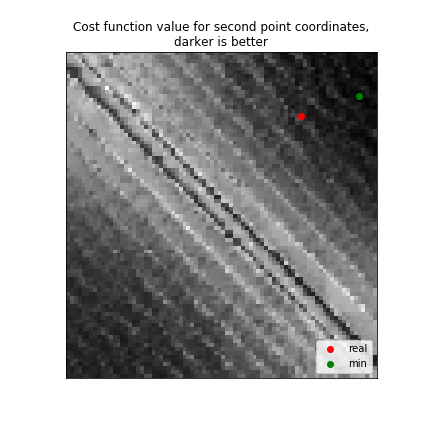
\includegraphics[width=0.5\linewidth]{cgrid-optimization_useless_x4}
	\caption{Значения целевой функции в зависимости от координат второй точки кривой}
	\label{fig:costFunctionGrid}
\end{figure}

Начальное приближение $B_1$ будем искать на серединном перпендикуляре между $B_0$ и $B_2$. Так это данная задача одномерной минимизации, допустимо применение метода перебора по дискретной сетке с достаточно малым шагом $\alpha$ среди точек $B_1^i = \alpha i \vec{n}+\frac{B_0+B_2}{2}$, где $i = \pm 1, \pm 2, \dots$, а $\vec{n}$~--- вектор нормали к прямой $B_0,B_2$.

\subsection{Уточнение параметров}
Для качественного восстановления изображения необходимо получить как можно более более точную оценку параметров искажения. Для чего применим метод градиентного спуска, начиная с полученных ранее оценок значений. Полученный таким образом минимум целевой функции может сойтись в глобальном минимуме, как следствие получим качественно восстановленное изображение.

Метод наискорейшего спуска:
\begin{enumerate}
	\item Задать начальное приближение $X_0$
	\item Рассчитать $X_{j+1} = X_j + \lambda_j \nabla F(X_j)$, где $\lambda_j = \argmin_{\lambda} (F(X_j) - \lambda\nabla F(X_j))$
	\item Если $|X_{j+1}-X_j| > \varepsilon$, то $j = j+1$, иначе $X = X_j$ и останов.
\end{enumerate}

Так как целевая функция зашумлена, здесь вместо градиента $\nabla F(x,y) = \left(\frac{\partial F(x,y)}{\partial x}, \frac{\partial F(x,y)}{\partial y}\right)$, воспользуемся дискретный приближением градиента~--- оператором Собеля. Так его компонента по x:
\begin{equation*}
	\begin{aligned}
		G_x(x,y) = &-F(x-1, y-1) - 2F(x-1, y) - F(x-1, y+1) + \\
                   &+F(x+1, y-1) + 2F(x+1, y) + F(x+1, y+1)
	\end{aligned}
\end{equation*}
Таким образом можно получить достаточно точную оценку искажающего оператора, если он не является слишком сложной кривой.

Итоговый алгоритм оценки параметров искажения:
\begin{algorithm} Определение параметров криволинейного искажающего оператора
	
	\textbf{Входные данные:} искажённое изображение

	\textbf{Выходные данные:} оценка параметров искажающего оператора $h(x,y)$, а именно точки кривой Безье $B_0, B_1, B_2$.
	\begin{enumerate}
		\item Зафиксировать точку $B_0 = (0;0)$;
		\item Вычислить кепстр $\hat{g}(x,y)$ искажённого изображения;
		\item Прибавить к кепстру ядро гаусса $gauss(x,y) = \frac{1}{\sigma\sqrt{2\pi}}e^{-\frac{x^2+y^2}{2\sigma^2}}$;
		\item Начальное приближение точки $B_2^0 = \argmin_{b=(x,y)} \left(\hat{g}(x,y) + gauss(x,y)\right)$;
		\item Начально приближение точки $B_1$ выбирается перебором на серединном перпендикуляре между $B_0$ и $B_2$;
		\item Последовательное уточнение точек $B_1$ и $B_2$ методом наикратчайшего спуска. 
	\end{enumerate}
	\label{algo:curve}
\end{algorithm}

\section{Выводы}
Были рассмотрены методы оценки параметров линейного и криволинейного искажающего оператора. Для каждого были сделаны выводы:
\begin{itemize}
	\item Для деконволюции предлагается использовать модифицированный метод Люси-Ричардсона;
	\item кепстр позволяет достаточно точно определить параметры линейного искажающего оператора;
	\item по кепстру также можно сделать первое приближение третьей точки криволинейного искажающего оператора;
	\item составлен алгоритм оценки параметров искажения.
\end{itemize}